\section{正迁移与负迁移}\label{sec:cross-domain-transfer}

相同的词元归一化形式在 PTB 和 WikiText-2 上产生正迁移，在 TinyStories 上产生负迁移（表~\ref{tab:cross_domain_transfer}；图~\ref{fig:cross_domain_gain}）。每个领域的三个独立学生准备结果都具有一致的增益方向。在 TinyStories 上，CE 在全部三个种子中都优于 $S_0$，因此有害的 KD 是相对于有效的续训而言，而不是两个无需进行的训练分支之间的比较。

这些结果确立了所测试配置下的可重复性，但不构成语料效应的因果证据。不同领域的教师、数据量与学生准备过程不同。纳入分析的终点均为有限值；梯度裁剪与偶发的 AMP 更新跳过仍限制了从优化角度进行解释（附录~\ref{app:protocols}）。完整的终点 NLL 与各种子的增益见附录~\ref{app:per-seed}。

\begin{table}[t]
\centering
\begin{tabular}{lrr}
\toprule
数据集 & 增益（均值 $\pm$ 标准差） & 符号一致性\\
\midrule
PTB & $+0.144937\pm0.003938$ & 3/3 $+$\\
WikiText-2 & $+0.155665\pm0.007692$ & 3/3 $+$\\
TinyStories & $-0.107219\pm0.000415$ & 3/3 $-$\\
\bottomrule
\end{tabular}
\caption{每个语料上三个独立学生模型的配对测试集 NLL 增益；报告样本标准差，$\lambda=5$，$\tau=2$。两个分支均按验证集 NLL 选择检查点。}
\label{tab:cross_domain_transfer}
\end{table}

\begin{figure*}[!t]
\centering
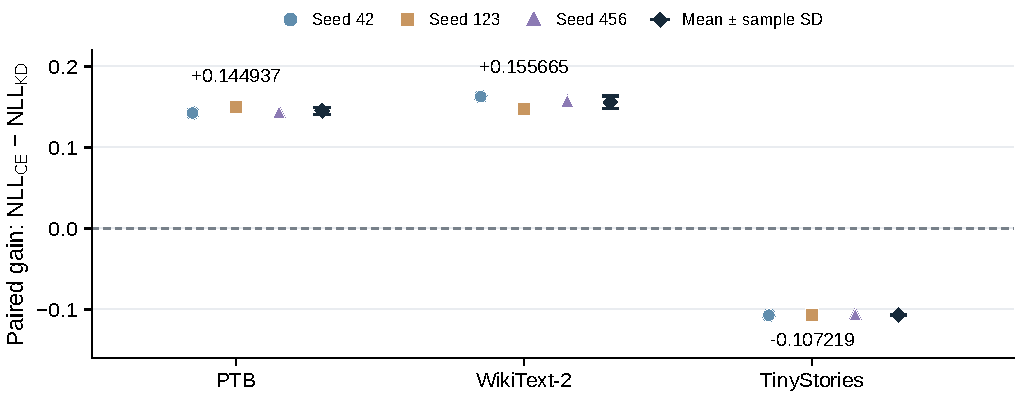
\includegraphics[width=\textwidth]{figures/fig2_cross_domain_gain.pdf}
\caption{相对于 CE 的测试 NLL 迁移结果。各散点表示独立的学生种子；黑色标记与误差条表示均值及样本 SD。正值表示 KD 更优。每个语料内部的教师与数据划分保持固定。}
\label{fig:cross_domain_gain}
\end{figure*}
